\documentclass[12pt]{article}


\usepackage{amssymb}
\usepackage{amsmath}
\usepackage{fullpage}
\usepackage{epsfig}
\usepackage{epstopdf}
\everymath{\displaystyle}

\newif\ifans

\ansfalse

\begin{document}

\begin{center}
\underline{\LARGE{The Fundamental Theorem of Calculus}}
\end{center}

\noindent SUGGESTED REFERENCE MATERIAL:
	
\bigskip

\noindent As you work through the problems listed below, you should reference Chapter 5.6 of the recommended textbook (or the equivalent chapter in your alternative textbook/online resource) and your lecture notes.

\bigskip

\noindent EXPECTED SKILLS:

\begin{itemize}

\item Be able to use one part of the Fundamental Theorem of Calculus (FTC) to evaluate definite integrals via antiderivatives. 

\item Know how to use another part of the FTC to compute derivatives of functions defined as integrals.

\end{itemize}

\noindent PRACTICE PROBLEMS:

\medskip

\begin{enumerate}

\item Consider the graph of $f(x)=\frac{1}{2}x-1$ on $[1,4]$, shown below.

\begin{center}

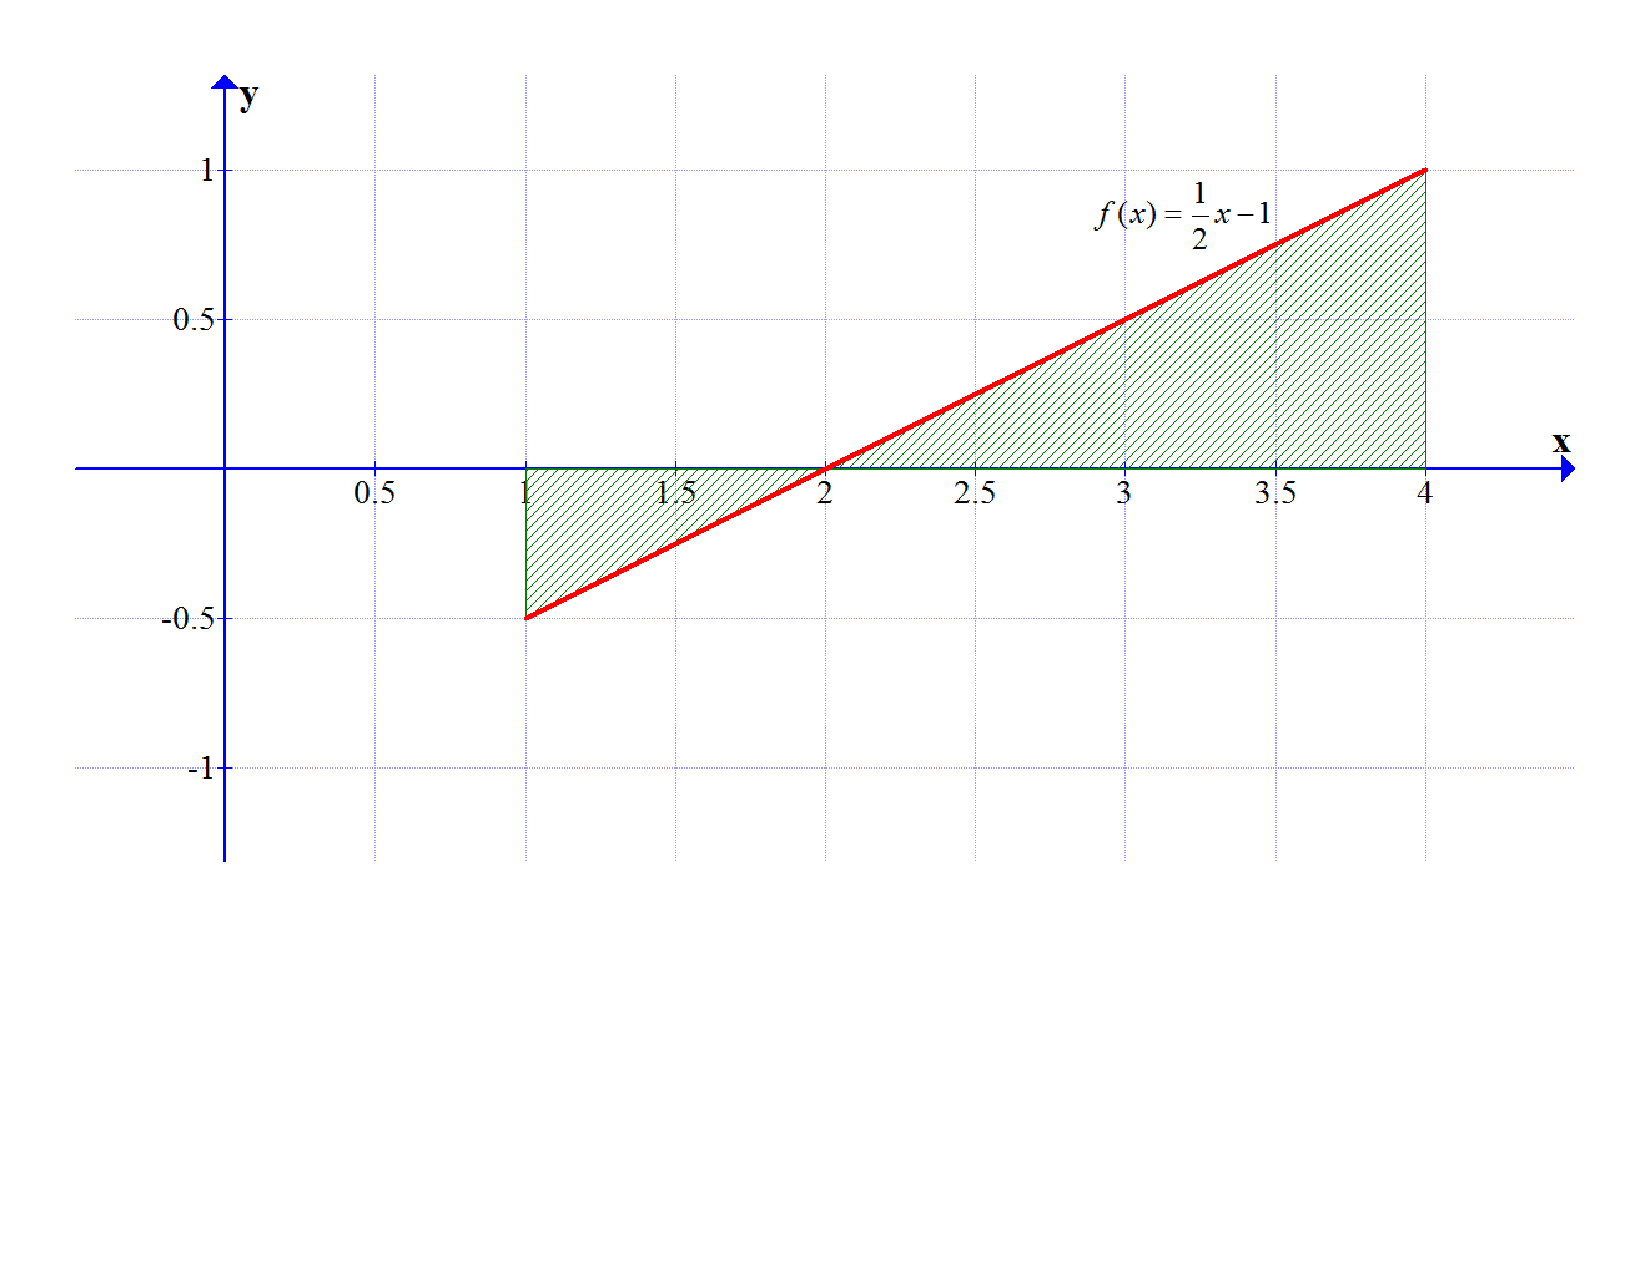
\includegraphics[scale=0.45]{area.pdf}

\end{center}

\begin{enumerate}

\item Use a definite intergal and the Fundamental Theorem of Calculus to compute the net signed area between the graph of $f(x)$ and the $x$-axis on the interval $[1,4]$.

\ifans{\fbox{$\int_1^4{\left(\frac{1}{2}x-1\right)}\,dx=\frac{3}{4}$}} \fi

\item Verify your answer from part (a) by using appropriate formulae from geometry.

\ifans{\fbox{\parbox{1\linewidth}{$A_{\text{lower triangle}}=\frac{1}{4}$; $A_{\text{upper triangle}}=1$;\\
 Thus, the value of the definite integral is $-A_{\text{lower triangle}}+A_{\text{upper triangle}}=\frac{3}{4}$}}} \fi

\end{enumerate}

\end{enumerate}

\newpage

\noindent {\bf For problems 2-4, sketch a region whose net signed area is equivalent to the value of the given definite integral.  Then  evaluate the definite integral using any method.}

\begin{enumerate}
\setcounter{enumi}{1}

\item $\int_0^8{(x^2-4x-5)}\,dx$

\ifans{\fbox{\parbox{1\linewidth}{\begin{center}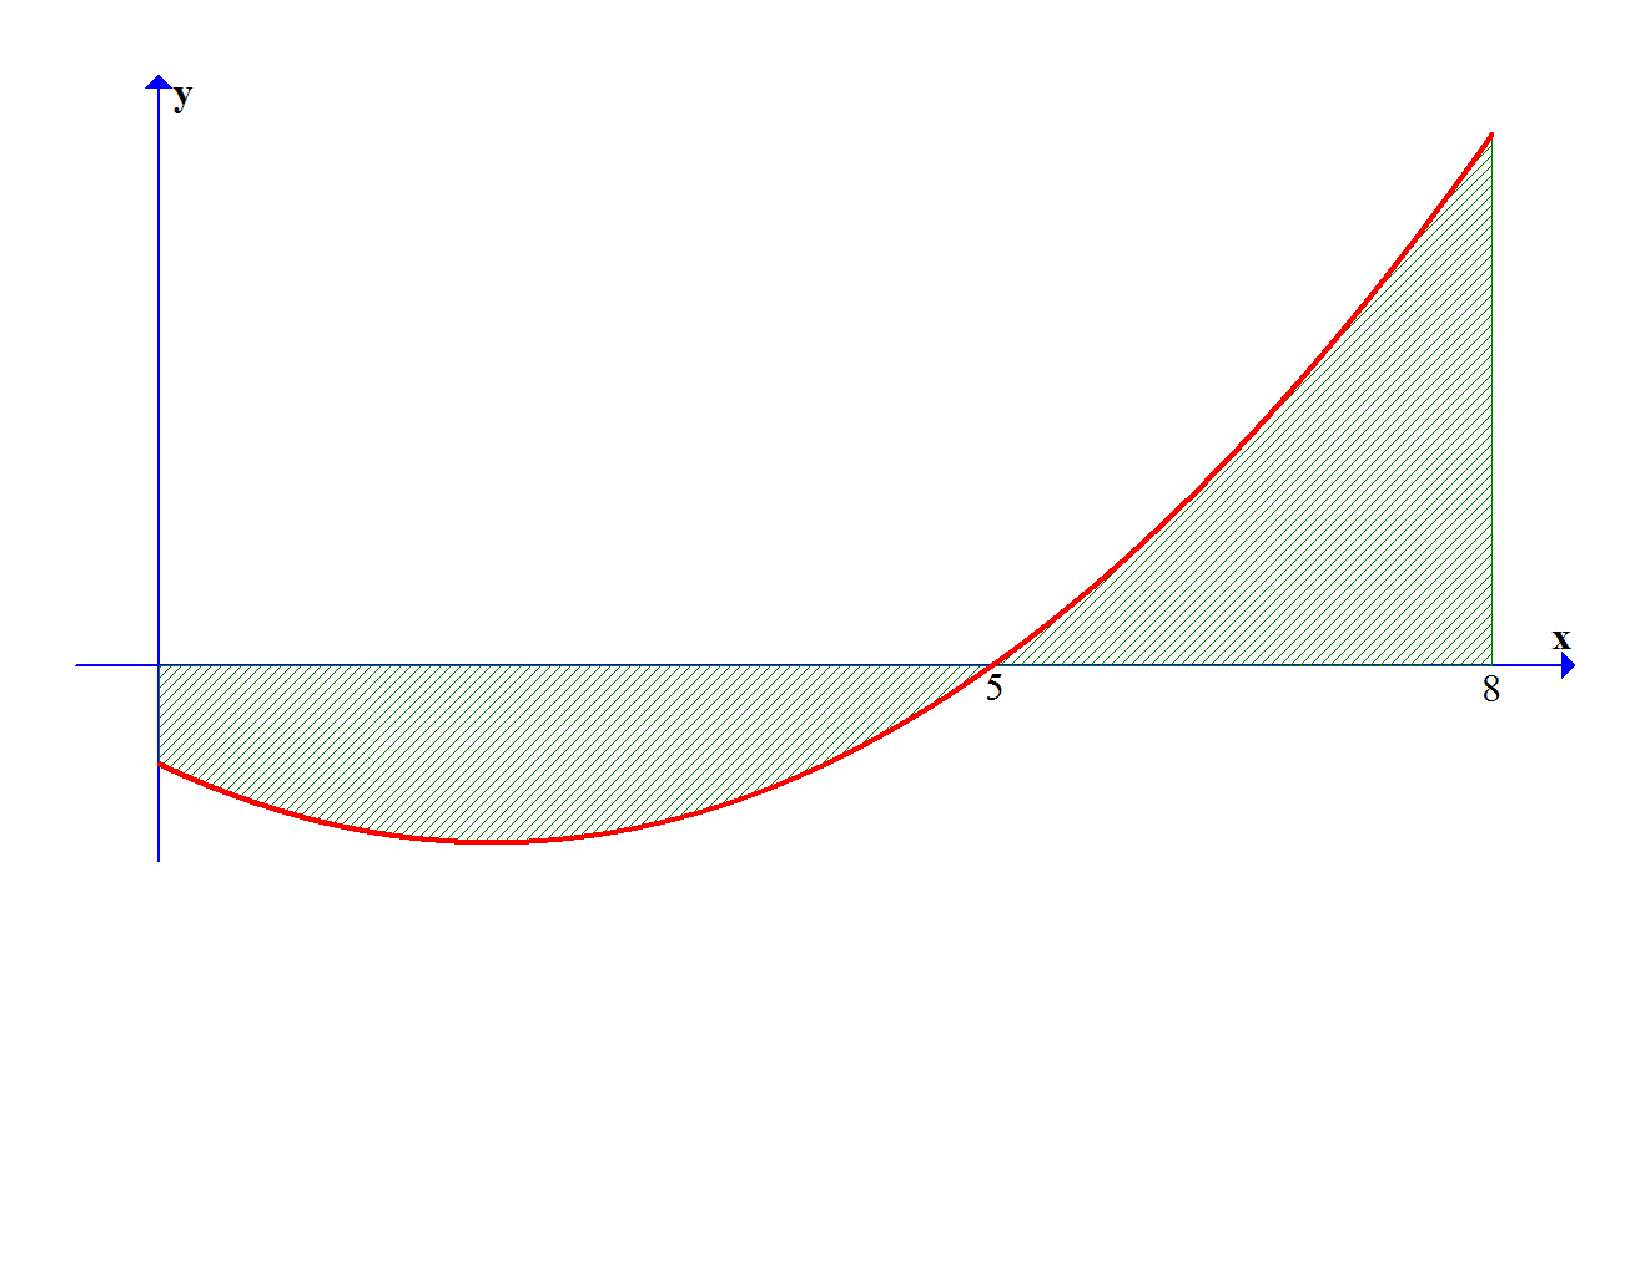
\includegraphics[scale=0.2]{2.pdf}\\
$\int_0^8(x^2-4x-5) \,dx=\frac{8}{3}$\end{center}}}} \fi

\item $\int_{\frac{\pi}{2}}^{\frac{3\pi}{2}}\cos{x} \,dx$

\ifans{\fbox{\parbox{1\linewidth}{\begin{center}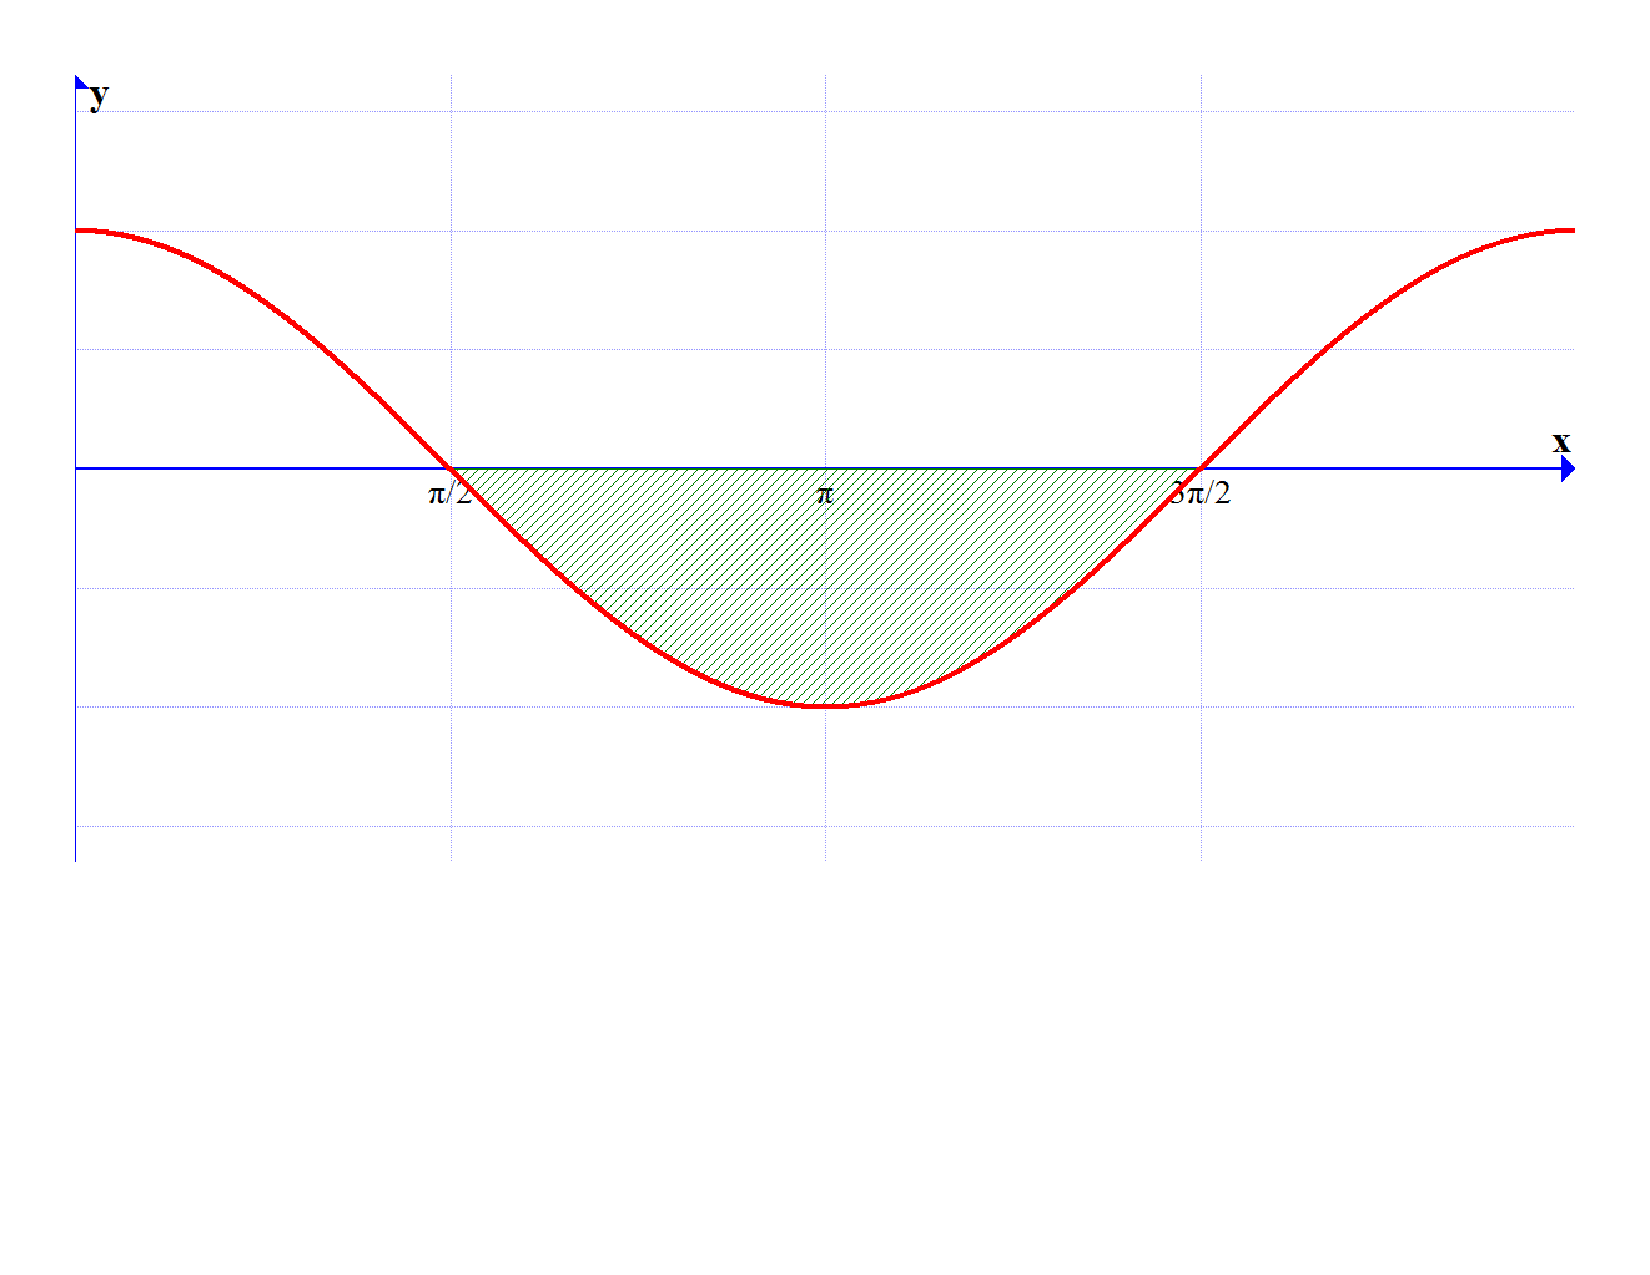
\includegraphics[scale=0.2]{3.pdf}\\
$\int_{\frac{\pi}{2}}^{\frac{3\pi}{2}}{\cos{x}} \,dx=-2$\end{center}}}} \fi

\item $\int_{-4}^{-1}\frac{2}{x^3}\,dx$

\ifans{\fbox{\parbox{1\linewidth}{\begin{center}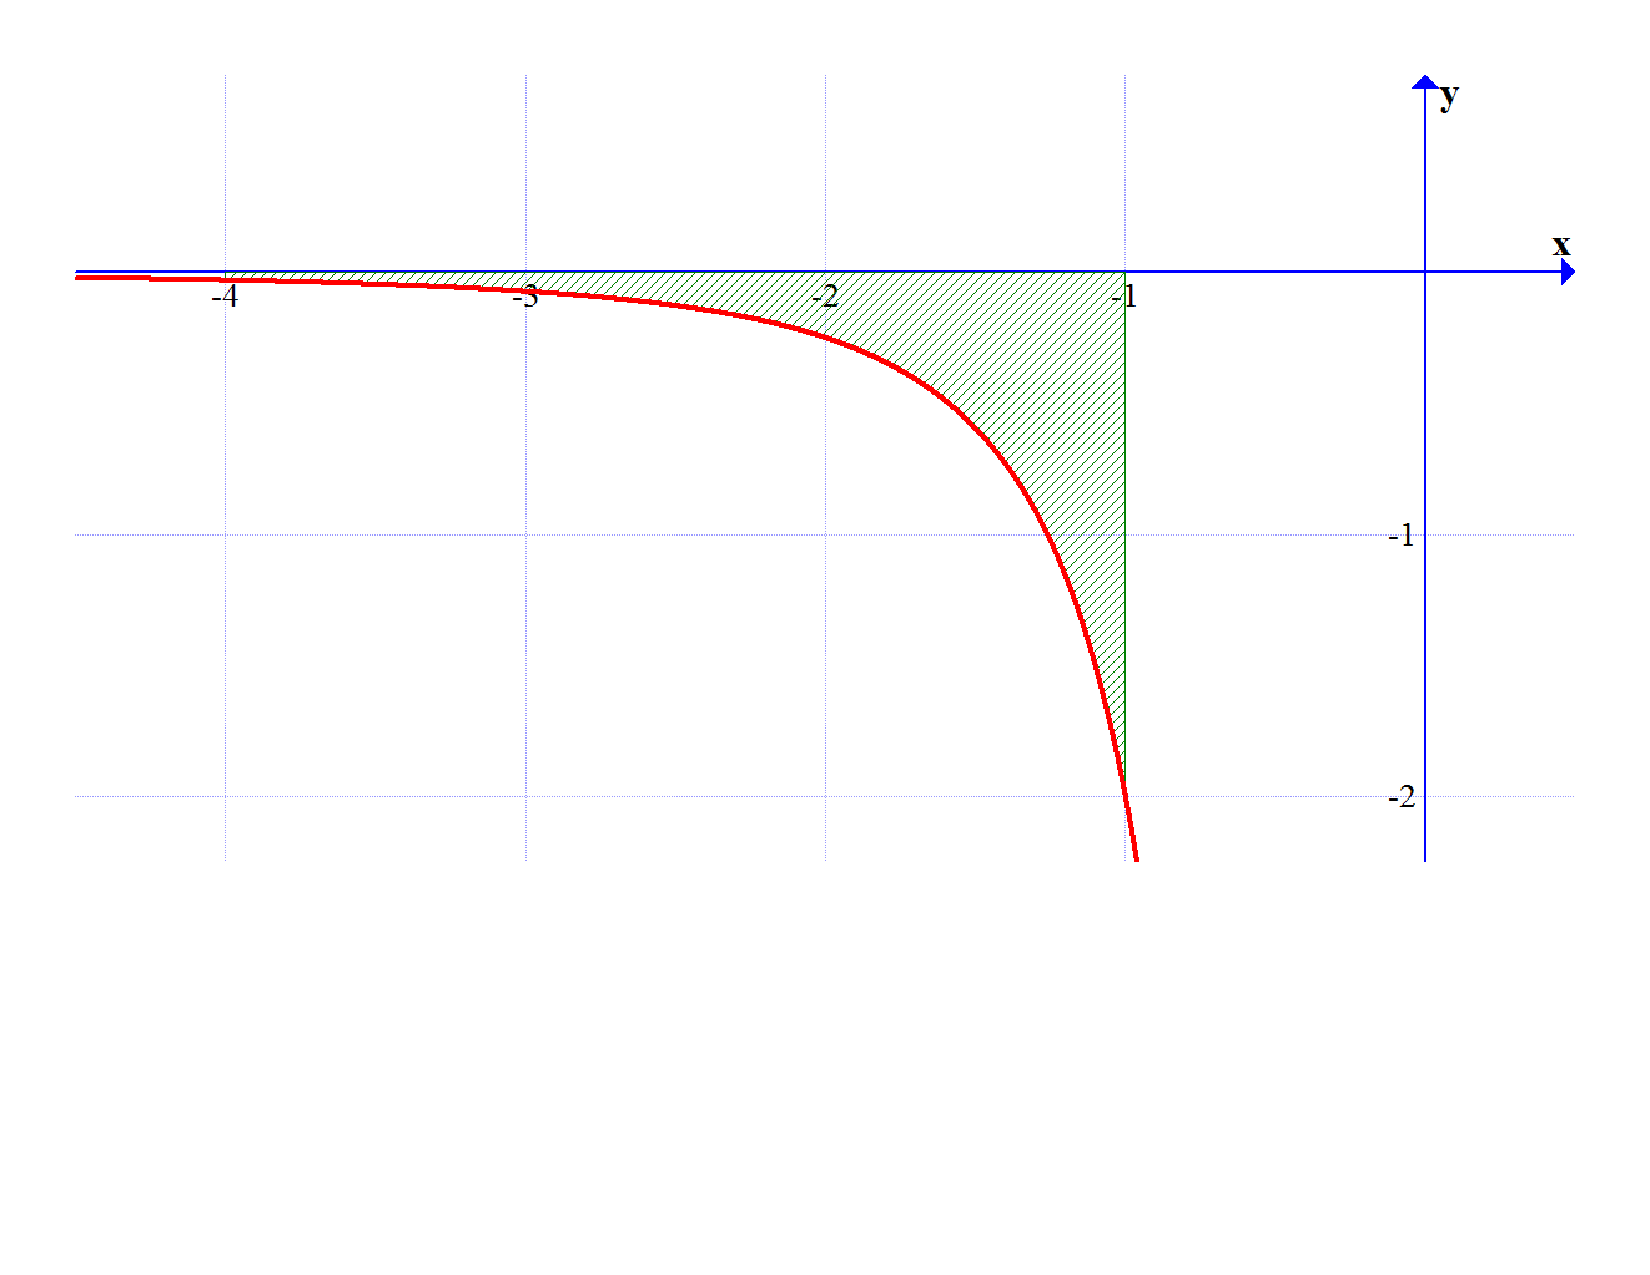
\includegraphics[scale=0.2]{4.pdf}\\
$\int_{-4}^{-1}{\frac{2}{x^3}} \,dx=-\frac{15}{16}$\end{center}}}} \fi

\end{enumerate}

\noindent {\bf For problems 5-15, evaluate the given definite integral.}

\begin{enumerate}
\setcounter{enumi}{4}

\item $\int\limits_{4}^{25} \frac{1}{x\sqrt{x}}\,dx$ 

\ifans{\fbox{$\frac{3}{5}$}} \fi

\item $\int_{-e}^{-1}{\frac{x+1}{x}} \,dx$

\ifans{\fbox{$-2+e$}} \fi

\item $\int_{\ln{2}}^{\ln{3}}e^{2x} \,dx$

\ifans{\fbox{$\frac{5}{2}$}} \fi

\item $\int\limits_{\frac{\pi}{2}}^{\frac{2\pi}{3}}\csc{(x)}\cot{(x)}\,dx$ 

\ifans{\fbox{$1-\frac{2}{\sqrt{3}}$}} \fi

\item $\int\limits_{0}^{\sqrt{3}}\frac{3}{1+x^2}\,dx$ 

\ifans{\fbox{$\pi$}} \fi

\item $\int\limits_{-9}^{9}|x-5|\,dx$ 

\ifans{\fbox{106}} \fi

\item $\int\limits^{e^{6}}_{1}\frac{1}{10 x}\,dx$ 

\ifans{\fbox{$\frac{3}{5}$}} \fi

\item $\int_{\frac{1}{\sqrt{2}}}^{\frac{\sqrt{3}}{2}} \frac{1}{\sqrt{1-x^2}} \,dx$ 

\ifans{\fbox{$\frac{\pi}{12}$}} \fi

\item $\int_{0}^{\pi} |\cos{x}| \,dx$

\ifans{\fbox{2}} \fi

\item $\int_0^3 f(x) \,dx$ if $f(x)=\left\{\begin{array}{lll}
x+5 & \text{  if} & x \leq 1\\
4x+2 & \text{  if} & x > 1
\end{array}\right.$

\ifans{\fbox{$\frac{47}{2}$}} \fi

\item $\int_0^{\frac{\pi}{4}} \tan^2{x} \,dx$.  (HINT: Use a trigonometric identity first to rewrite the integrand.)

\ifans{\fbox{$1-\frac{\pi}{4}$}} \fi

\item \fbox{\bf Definitions:} If an object moves along a straight line with position function $s(t)$, its velocity function is $v(t)=s^{\prime}(t)$.  Then:

\begin{itemize}

\item The \underline{displacement} from time $t_1$ to time $t_2$ is the net change of position of the particle during the time period from $t_1$ to $t_2$ and is calculated by evaluating$\int_{t_1}^{t_2} v(t) \,dt$.

\item The \underline{total distance traveled} from time $t_1$ to time $t_2$ is calculated by evaluating $\int_{t_1}^{t_2} |v(t)| \,dt$.

\end{itemize}

Assume that a particle is moving along a straight line such that its velocity at time $t$ is $v(t)=t^2-6t+5$  (meters per second).  
\begin{enumerate}

\item Compute the displacement of the particle during the time period $0 \leq t \leq 6$.

\ifans{\fbox{$-6$ meters}} \fi

\item Compute the total distance traveled by the particle during the time period $0 \leq t \leq 6$.

\ifans{\fbox{$\frac{46}{3}$ meters}} \fi

\end{enumerate}

\item The following Riemann Sum was derived by dividing an interval $[a,b]$ into $n$ subintervals of equal width and then choosing $x_k^*$ to be the right endpoint of each subinterval.

$$\lim_{n \rightarrow +\infty} \sum_{k=1}^n{\left(1+\frac{4}{n}k\right)\frac{4}{n}}$$

\begin{enumerate}

\item What is the interval, $[a,b]$?

\ifans{\fbox{If we consider $f(x)=x$, then the interval is $[1,5]$}} \fi

\item Convert the Riemann Sum to an equivalent definite integral.

\ifans{\fbox{$\lim_{n \rightarrow +\infty} \sum_{k=1}^n{\left(1+\frac{4}{n}k\right)\frac{4}{n}}=\int_1^5{x} \,dx$}} \fi

\item Using the definite integral from part (b) and part of the Fundamental Theorem of Calculus, evaluate the limit.

\ifans{\fbox{12}} \fi

\end{enumerate}

\ifans{{\bf NOTE:} In number 17, we could have considered $f(x)=1+x$.  In that case, $[a,b]=[0,4]$ and $\lim_{n \rightarrow +\infty} \sum_{k=1}^n{\left(1+\frac{4}{n}k\right)\frac{4}{n}}=\int_0^4{(1+x)} \,dx$.  The value of this definite integral is also 12.} \fi

\item Explain what is wrong with the following calculation:

$$\int_{-1}^1 \frac{1}{x^2} \,dx =\left. -\frac{1}{x}\right|_{x=-1}^{x=1}=-1-(1)=-2$$

\ifans{\fbox{\parbox{1\linewidth}{$f(x)=\frac{1}{x^2}$ is not continuous at $x=0$ which is in $[-1,1]$; so, the FTC does not immediately apply.}}} \fi

\end{enumerate}

\noindent {\bf For problems 19-22, use part of the Fundamental Theorem of Calculus to compute the indicated derivative.}

\begin{enumerate}
\setcounter{enumi}{18}

\item $\frac{d}{dx}\int\limits_{2}^{x} \ln{(t)} \,dt$ 

\ifans{\fbox{$\ln{(x)}$}} \fi

\item $\frac{d}{dx}\int\limits_{x}^{10} e^{t^2} \,dt$ 

\ifans{\fbox{$-e^{x^2}$}} \fi

\item $\frac{d}{dx}\int\limits_{\pi}^{3x^2} \cos{t} \,dt$ 

\ifans{\fbox{$6x\cos{\left(3x^2\right)}$}} \fi

\item $\frac{d}{dx}\int\limits_{2}^{e^x} \ln{(t)} \,dt$ 

\ifans{\fbox{$xe^x$}} \fi

\item Consider $F(x)=\int_4^x{\sqrt[3]{t^2+11}} \,dt$. Compute each of the following:

\begin{enumerate}

\item $F(4)$

\ifans{\fbox{$0$}} \fi

\item $F^{\prime}(4)$

\ifans{\fbox{$3$}} \fi

\item $F^{\prime \prime}(4)$

\ifans{\fbox{$\frac{8}{27}$}} \fi

\end{enumerate}

\item Let $F(x)=\int_1^x t\ln{t} \,dt$, for $x>0$.

\begin{enumerate}

\item Find the open interval(s) on which $F(x)$ is increasing and those on which $F(x)$ is decreasing.

\ifans{\fbox{$F(x)$ is increasing on $(1,\infty)$ and is decreasing on $(0,1)$.}} \fi

\item Find all points $(x,y)$ where the graph of $F(x)$ has a local (relative) maximum or a local (relative) minimum.

\ifans{\fbox{$F(x)$ has a local minimum at $(1,0)$ and does not have any local maxima.}} \fi

\item Find the interval(s) on which $F(x)$ is concave up and those on which $F(x)$ is concave down.

\ifans{\fbox{$F(x)$ is concave down on $\left(0,\frac{1}{e}\right)$ and is concave up on $\left(\frac{1}{e},\infty\right)$}} \fi

\item Determine the $x$-value(s) of each inflection point of $F(x)$.

\ifans{\fbox{$F(x)$ has an inflection point when $x=\frac{1}{e}$}} \fi

\end{enumerate}

\end{enumerate}

\end{document}